\chapter{浮动体}
\label{cha:float}
本章将介绍本模板的浮动体,包括表格、插图以及算法环境。
\section{三线表}
\label{sec:sheet}
三线表是论文写作中常见的表格形式,一般的表格如表\ref{tab:siftflow}所示:
\begin{table}[h] 
	\renewcommand\arraystretch{1.5}
	\centering
		\bicaption{典型的实验对比表格}{Typical experimental comparison table}
		\begin{tabular}{*{4}{c}}
			\toprule
	 		Method & Pixel Acc. & Mean Acc. & Mean Iu.\\
			\midrule
			Liu等人\cite{liu2011sift}  & 76.7 & - & -\\
			Tighe等人\cite{tighe2013finding}  & 78.6 & 39.2 & -\\
			FCN-16s\cite{long2015fully} & 85.2 & 51.7 & 39.5\\
			Deeplab-LargeFOV\cite{chen14semantic} & 85.6 & 51.2 & 39.7\\
			\midrule
			Grid-LSTM5 & 86.2 & 51.0 & 41.2\\
			\bottomrule
		\end{tabular}	
		\label{tab:siftflow}
\end{table}

较为复杂的表格:
\begin{table}[h]
	\renewcommand\arraystretch{1.5}
	\centering
	\bicaption{较为复杂的表格(涉及单元格的合并与拆分)}{Relatively complex tables (involving merging and splitting of cells)}
	\begin{tabular}{*{5}{c}}
		\toprule
		区域 & \tabincell{c}{外侧核热功率\\(MW)} & \tabincell{c}{内侧核热功率\\(MW)} & 结构 & \tabincell{c}{结构核热功率\\(MW)} \\
		\midrule
		第一壁涂层 & 20.0 & 13.4 & \multirow{2}{*}{第一壁} & \multirow{2}{*}{151.7} \\
		第一壁结构层 & 70.2 & 48.1 & ~ & ~ \\
		\midrule
		Be-1区 & 37.9 & 26.5 & \multirow{4}{*}{氚增殖区} & \multirow{4}{*}{736.2} \\ 
		Li$ _{\text{4}} $SiO$ _{\text{4}} $-1区 & 126.7 & 86.8 & ~ & ~ \\
		Be-2区 & 133.6 & 94.1 & ~ & ~ \\
		Li$ _{\text{4}} $SiO$ _{\text{4}} $-2区 & 134.4 & 96.2 & ~ & ~ \\
		\bottomrule
	\end{tabular}
	\label{tab:nucheat_tot}
\end{table}

编制表格应简单明了,表达一致,明晰易懂,表文呼应、内容一致。排版时表格字号略小,或变换字体,尽量不分页,尽量不跨节。表格太大需要转页时,需要在续表上方注明“续表”,表头页应重复排出。

\section{插图}
\label{sec:figure}
有些人可能听说“\LaTeX 只能使用 eps 格式的图片”,甚至把 jpg 格式转为 eps。事实上,这种做法已经过时。而且每次编译时都要要调用外部工具解析 eps,导致降低编译速度。所以我们推荐矢量图直接使用 pdf 格式,位图使用 jpeg 或 png 格式。
\begin{figure}[h] 
	\centering
	\includegraphics[width=0.45\textwidth]{image/confusion.pdf}
	% \bicaption{图片插入示例}{Example of inserting figures}
	\bicaptionX{图片插入示例}{Example of inserting figures}
	\label{fig:confusion}
\end{figure}

关于图片的并排,推荐使用较新的 subcaption 宏包,不建议使用 subfigure 或 subfig 等宏包,但对于多张图片还是不宜使用\LaTeX 直接插入,应将所需插入的图片先用PowerPoint排列、拼接,再标号,生成一张图片,再整个插入论文中。

有些时候图片会有比较复杂的信息需要进一步解释(例如图片中包括不同的子图,或者图片中不同元素的具体含义)。
而这些详细的图/表注释信息不需要出现在文档开始的图表目录中。
这里本模板提供了\verb|\bicaptionX|命令用于自动排版注释内容,效果如图\ref{fig:sponge}。为了和注释区分,这一命令会自动在正文中对标题进行加粗。

\begin{figure}[h] 
	\centering
	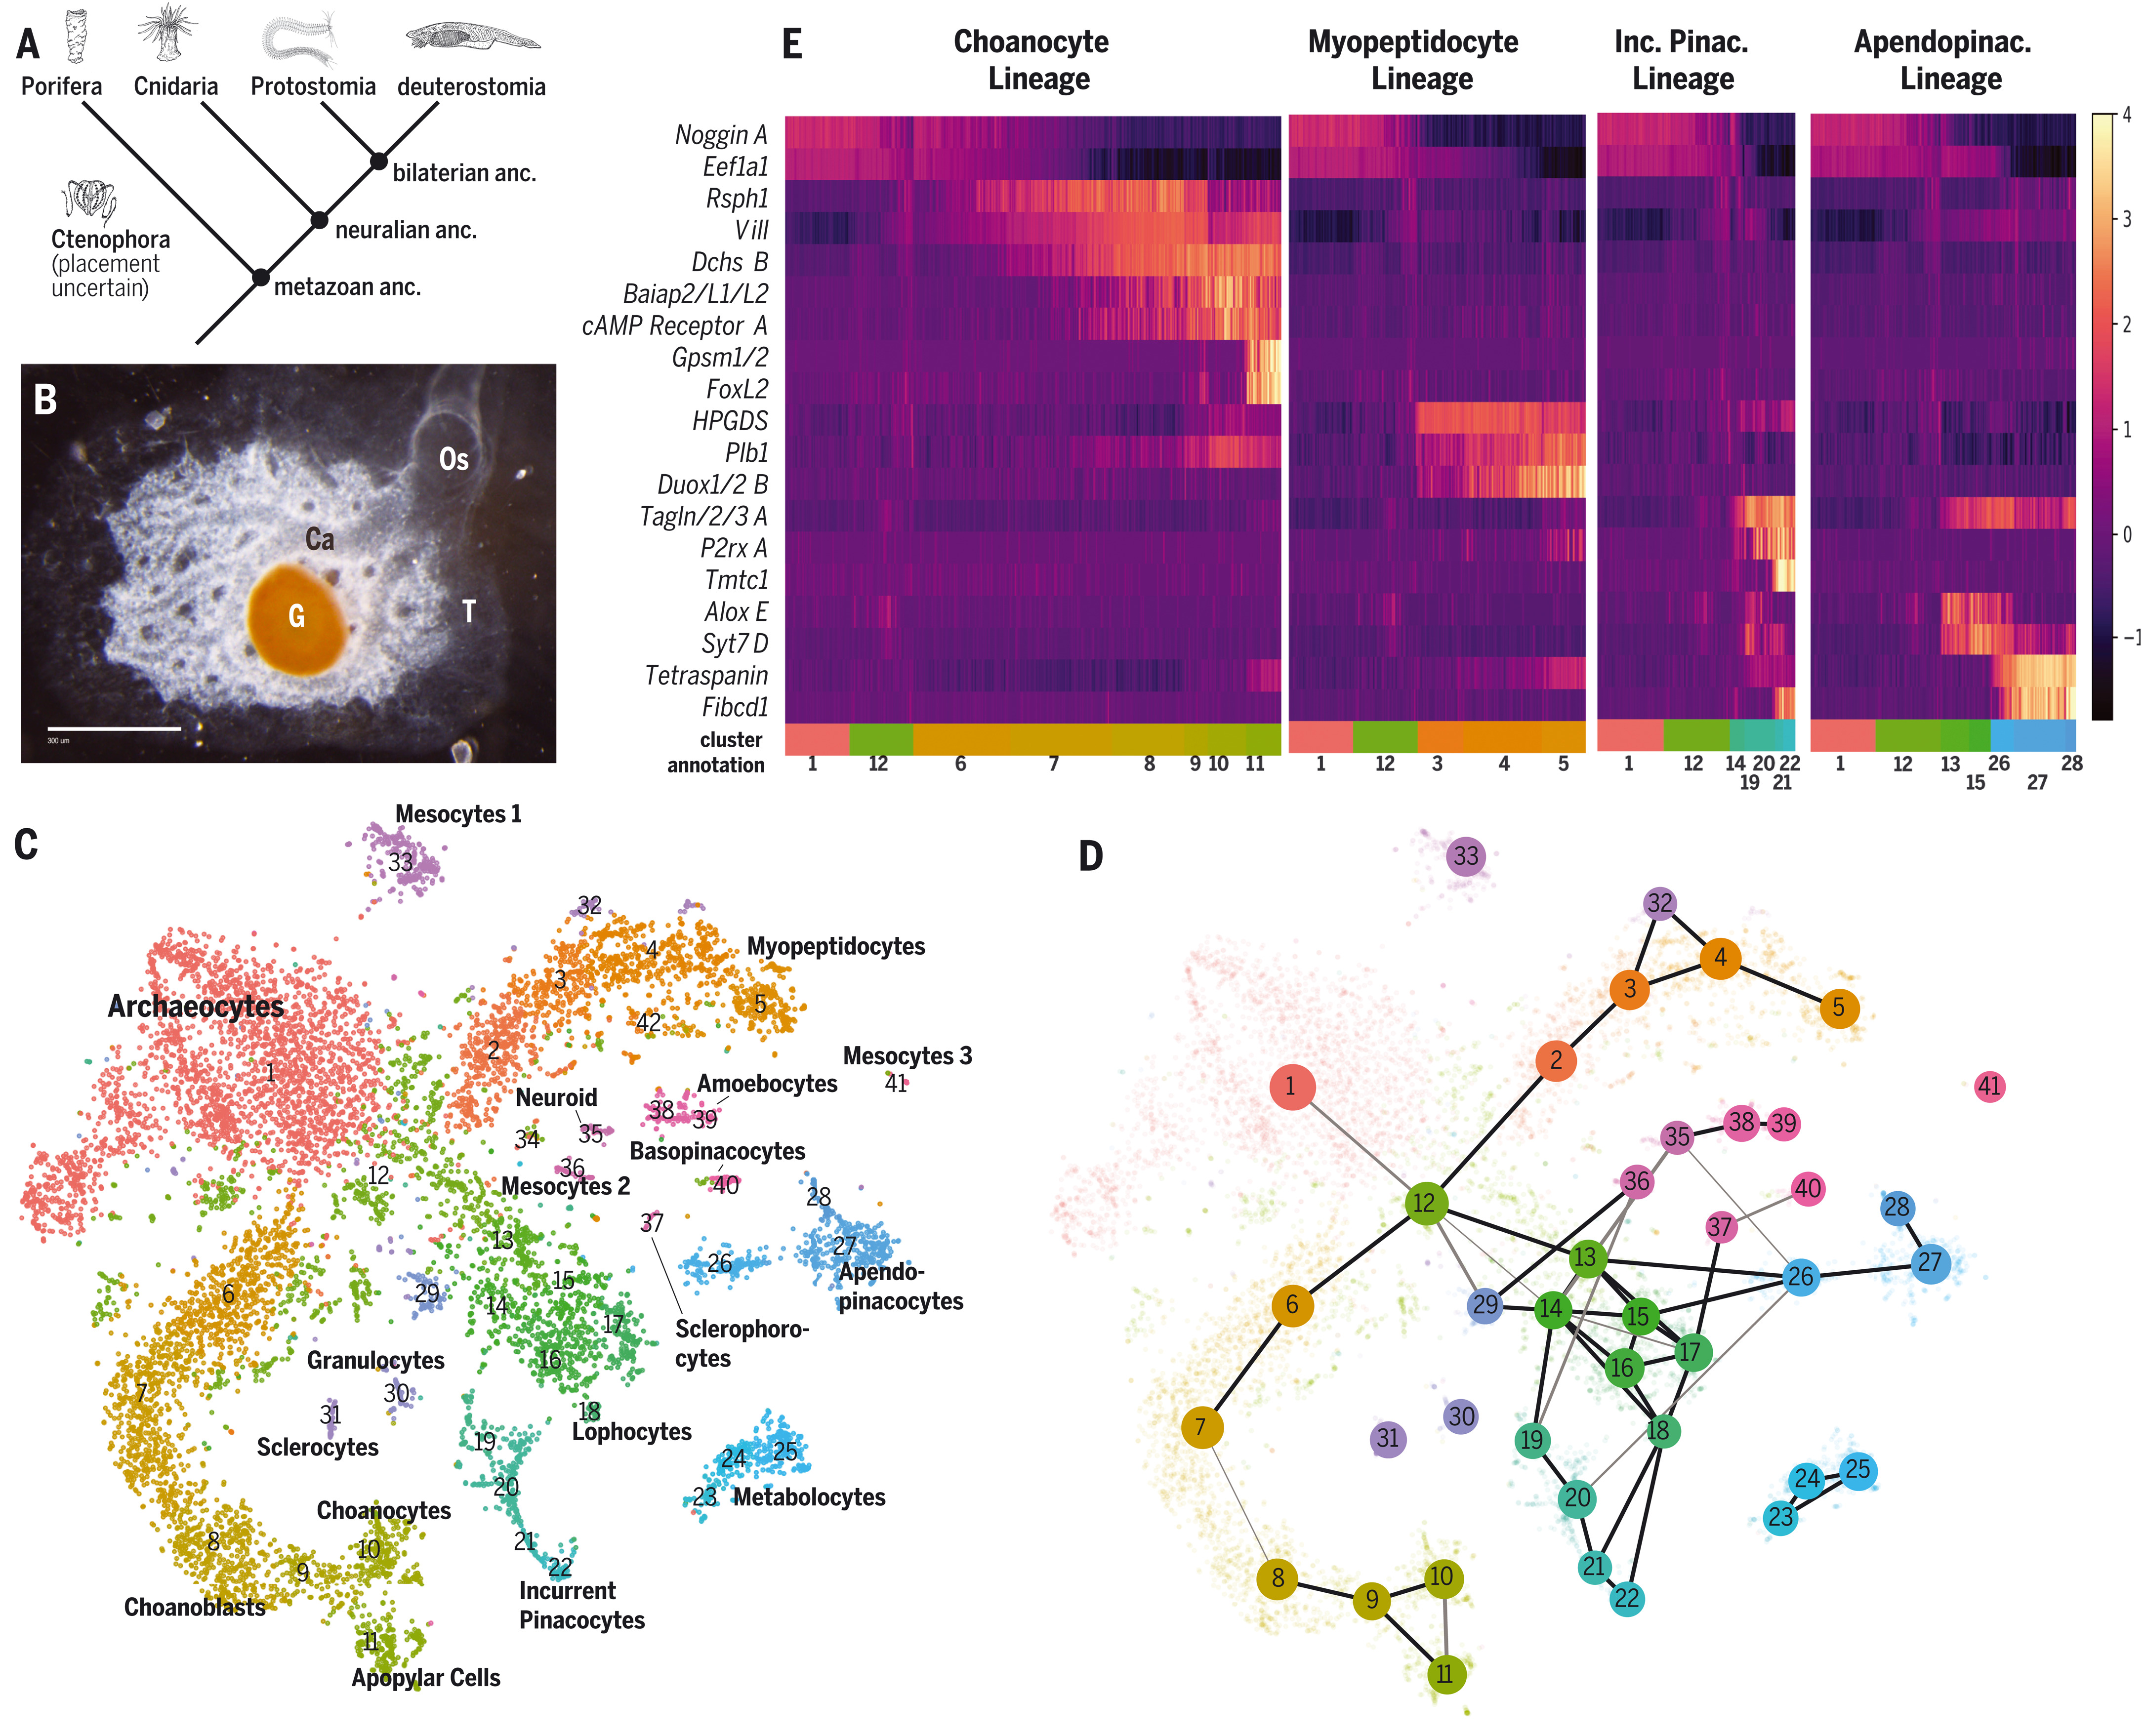
\includegraphics[width=0.7\textwidth]{image/sponge-celltype.jpg}
	% \bicaption{图片插入示例}{Example of inserting figures}
	\bicaptionX{复杂图片注释示例}{Example of complex image annotation}{(\textbf{A})动物祖先系统发育树。(\textbf{B})\textit{S.lacustris}鸟瞰图。(\textbf{C})10106 个细胞组成的 TSNE 图,颜色表示42个不同聚类。(\textbf{D})PAGA 连接图,边的粗细代表连接强度,节点尺寸代表细胞数量。(\textbf{E}) PAGA 路径的差异表达标记的归一化表达值。图片引自\cite{musser2021}。}
	\label{fig:sponge}
\end{figure}

其基本使用方法为:

\begin{verbatim}
	没有注释:
	\bicaptionX{中文标题}{English Title}
	有注释:
	\bicaptionX{中文标题}{English Title}{注释}	
\end{verbatim}

如果对这一实现不够满意,也可以自行查阅 bicaption 宏包的\href{https://sg.mirrors.cicku.me/ctan/macros/latex/contrib/caption/bicaption.pdf}{文档}。

\section{算法环境}
\label{sec:algorithm}
模板中使用 algorithm2e 宏包实现算法环境。关于该宏包的具体用法,请阅读宏包的官方文档。

\normalem
\begin{algorithm}[h]
	\SetAlgoLined
	\KwData{this text}
	\KwResult{how to write algorithm with \LaTeX2e }
  
	initialization\;
	\While{not at end of this document}{
	  read current\;
	  \eIf{understand}{
		go to next section\;
		current section becomes this one\;
	  }{
		go back to the beginning of current section\;
	  }
	}
	\caption{算法示例1}
	\label{algo:algorithm1}
  \end{algorithm}
  \ULforem

  注意,我们可以在论文中插入算法,但是不推荐在正文部分插入大段代码。